\chapter{Конструкторская часть}

% В данном разделе представлены этапы проектирования выделенных в предыдущем разделе баз данных, нужных для решения задачи.
\section{Функциональная модель}

На рисунке \ref{img:func_model} изображена функциональная модель, отображающая структуру и функции системы.

\begin{figure}[h!]
	\begin{center}
		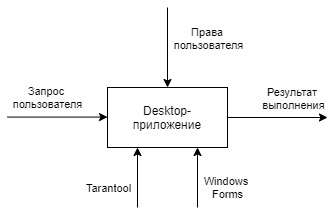
\includegraphics[scale=0.7]{../imgs/func_model.jpg}
	\end{center}
	\captionsetup{justification=centering}
	\caption{Функциональная модель приложения}
	\label{img:func_model}
\end{figure}









\section{Проектирование базы данных}




В соответствии с этой диаграммой база данных должна хранить следующие таблицы:  


\begin{itemize}
	\item таблица трасс slopes;
	\item таблица подъемников lifts;
	\item таблица связей трасс и подъемников lifts\_slopes;
	\item таблица турникетов turnstiles;
	\item таблица проездных карт cards;
	\item таблица считываний карт на турникетах подъемников card\_readings;
	\item таблица сообщений о происшествиях messages;
	\item таблица пользователей users.
	%\item таблица групп пользователей.
\end{itemize}


Таблица slopes хранит информацию о трассах и содержит следующие поля:
\begin{itemize}
	\item slope\_id -- уникальный идентификатор трассы, PK;
	\item slope\_name -- уникальное название;
	\item difficulty\_level -- уровень сложности;
	\item is\_open -- открыта или закрыта.
\end{itemize}


Таблица lifts хранит информацию о подъемниках и содержит следующие поля:
\begin{itemize}
	\item lift\_id -- уникальный идентификатор подъемника, PK;
	\item lift\_name -- уникальное название;
	\item is\_open -- открыт или закрыт;
	\item seats\_amount -- количество мест;
	\item lifting\_time -- время подъема;
	\item queue\_time -- время в очереди;
\end{itemize}


Эти две таблицы связаны отношением многие-ко-многим. Таблица lifts\_slopes хранит информацию об этих отношениях (связях трасс и подъемников) и содержит следующие поля:
\begin{itemize}
	\item record\_id -- уникальный идентификатор записи, PK;
	\item lift\_id -- идентификатор подъемника, FK на поле lift\_id таблицы lifts;
	\item slope\_id -- идентификатор трассы, FK на поле slope\_id таблицы slopes.
\end{itemize}


Таблица turnstiles хранит информацию о турникетах и содержит следующие поля:
\begin{itemize}
	\item turnstile\_id -- уникальный идентификатор турникета, PK;
	\item lift\_id -- идентификатор подъемника, FK на поле lift\_id таблицы lifts;
	\item is\_open -- открыт или закрыт.
\end{itemize}


Таблица cards хранит информацию о проездных картах и содержит следующие поля:
\begin{itemize}
	\item card\_id -- уникальный идентификатор карты, PK;
	\item activation\_time -- дата и время активации;
	\item type -- тип карты (детская, взрослая, временная, ...).
\end{itemize}


Таблица card\_readings хранит информацию о считываниях карт на турникетах подъемников и содержит следующие поля:
\begin{itemize}
	\item record\_id -- уникальный идентификатор считывания, PK;
	\item turnstile\_id -- идентификатор турникета, FK на поле turnstile\_id таблицы turnstiles;
	\item card\_id -- идентификатор проездной карты, FK на поле card\_id таблицы cards;
	\item reading\_time -- дата и время считывания.
\end{itemize}


Таблица users хранит информацию о пользователях и содержит следующие поля:
\begin{itemize}
	\item user\_id -- уникальный идентификатор пользователя, PK;
	\item card\_id -- идентификатор проездной карты (может отсутсвовать), FK на поле card\_id таблицы cards;
	\item user\_email -- адрес электронной почты (он же будет использоавться как логин);
	\item password -- пароль;
	\item permissions -- права доступа (роль).
\end{itemize}


Таблица messages хранит информацию о сообщениях пользователей о происшествиях и содержит следующие поля:
\begin{itemize}
	\item message\_id -- уникальный идентификатор сообщения, PK;
	\item sender\_id -- идентификатор отправителя, FK на поле user\_id таблицы usres;
	\item checked\_by\_id -- идентификатор прочитавшего, FK на поле user\_id таблицы usres;
	\item text -- текст сообщения.	
\end{itemize}



На рисунке \ref{img:db} предоставлена диаграмма реализованной базы данных.



\begin{figure}[h!]
	\begin{center}
		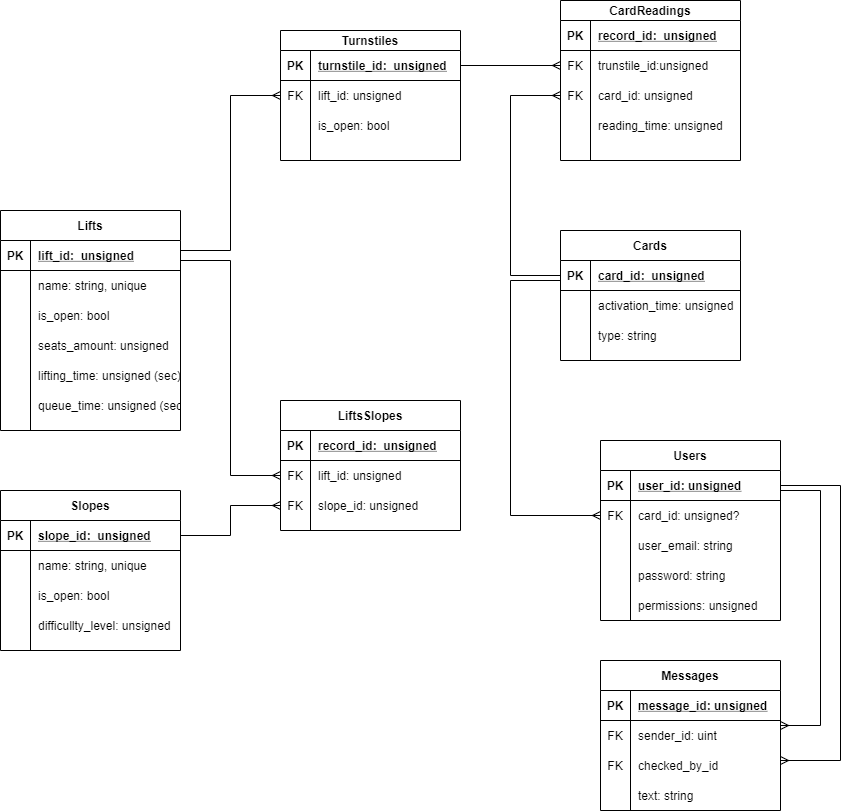
\includegraphics[scale=0.4]{../imgs/db/db.png}
	\end{center}
	\captionsetup{justification=centering}
	\caption{Диаграмма базы данных}
	\label{img:db}
\end{figure}
































